\documentclass{llncs}

\usepackage{graphicx}
\usepackage{caption}
\usepackage{subcaption}

\graphicspath{ {images/} }
%
\begin{document}

Online reviews for products, services, and places have become increasingly important resources for consumers to make informed decisions. Thus, it may be useful to detect which reviews are outstanding or anomalous in some way. For instance, fake reviews are harmful for the integrity of online reviewing systems, so they should be detected and removed. 

In this paper, I present a new method for detecting anomalous reviews using the opinions of product attributes (for example, battery life or picture quality). This method performs significantly better than using TF-IDF. Using product reviews injected with reviews of different products as test data, the method using opinion scores maintains a 100\% TPR while decreasing the FPR to 35\%.

The following describes the steps of the anomaly detection algorithm. The opinion extraction step is accomplished using a version of the algorithm in �A Holistic Lexicon-Based Approach to Opinion Mining� (Ding et al). The anomaly detection step using singular value decomposition is based on similar methods for computer networks from �Diagnosing Network-Wide Traffic Anomalies� (Lakhina et al).

\begin{enumerate}
\item Run the text of the product reviews (along with the corresponding product attributes per review, henceforth referred to as product �features�) through the opinion extraction algorithm, which will output the features with their opinion scores.
\item Construct an $n \times m$ data matrix for each product, where $n$ is the number of reviews for that product and $m$ is twice the number of features (one column for positive feature opinions and one column for negative feature opinions).
\item Perform singular value decomposition on the data matrix to get the singular value matrix $\Sigma$. Re-compute the data matrix using only the first $k$ singular values (where $k$ is the �knee� of the singular value data). Subtract this from the original data matrix to get the residual data matrix (this describes the noisy data). Compute the L2 norm for each row (review).
\item Classify each review as anomalous or normal using its L2 norm and a specified threshold.
\end{enumerate}

The above algorithm can only work if just a few singular values describe a majority of the reviews. Here I plotted the singular values of 4 products using binary feature values and real feature values. As Figure \ref{fig:sv} shows, all products, using binary or real valued features, have a �knee� in the data, which indicates that singular values above the knee describe most of the data, while singular values under the knee account for noisy data and anomalies.

In addition, using real-valued feature opinion scores often results in a sharper knee (more data is described by the first few singular values), so real values are a better way to distinguish between normal data and noisy/anomalous data. Using the L2 norm for the anomaly test is also appropriate, as Figure \ref{fig:l2norm-opinions} shows. The spikes in the plot indicate which reviews are anomalous.


\begin{figure}
\centering

	\begin{subfigure}{0.5\textwidth}
	\centering
	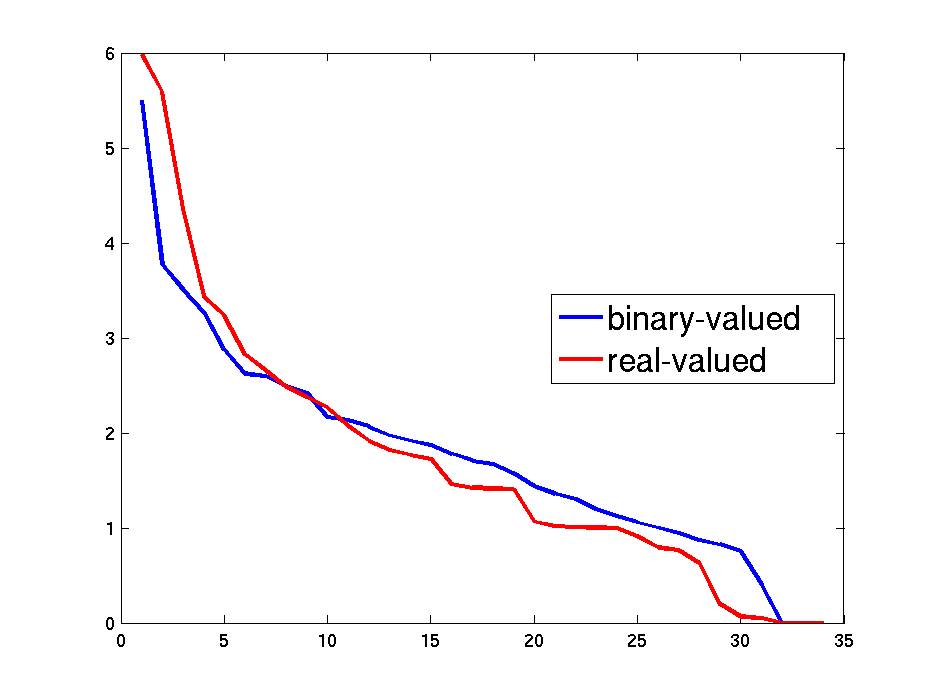
\includegraphics [scale=0.3]{sv-plot-nikon.png}
	\label{fig:sv-nikon}
	\end{subfigure}%
	~
	\begin{subfigure}{0.5\textwidth}
	\centering
	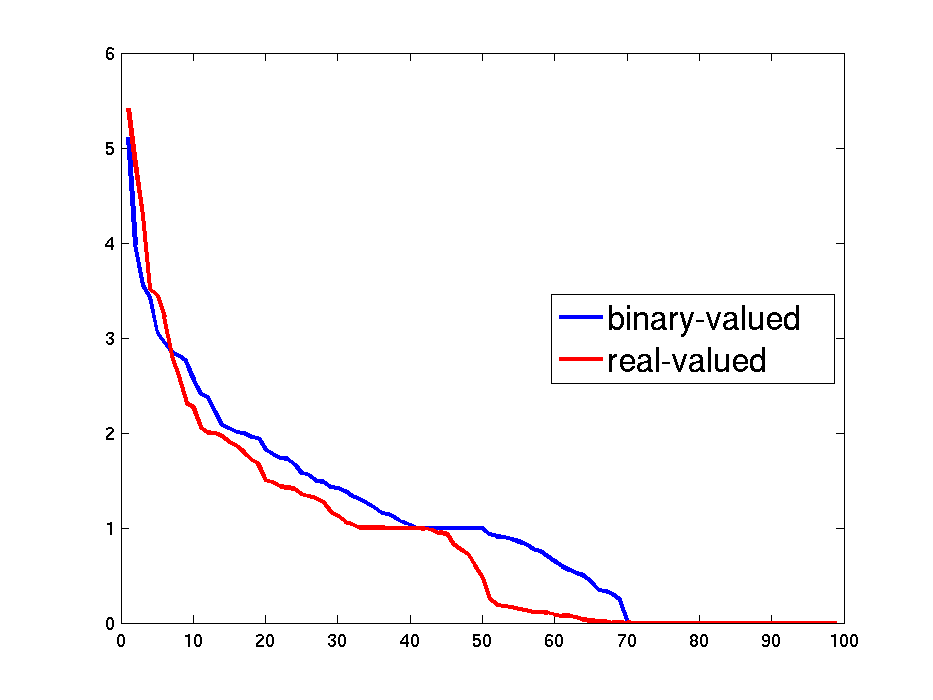
\includegraphics [scale=0.3] {sv-plot-apex.png}
	\label{fig:sv-apex}
	\end{subfigure}
	~
	\begin{subfigure}{0.5\textwidth}
	\centering
	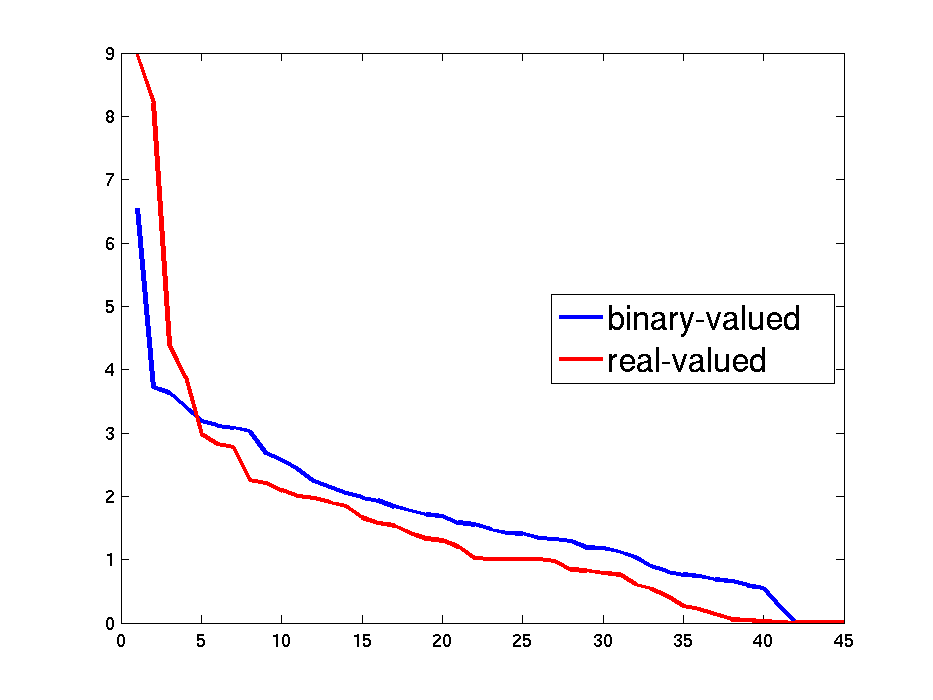
\includegraphics [scale=0.3] {sv-plot-canon.png}
	\label{fig:sv-canon}
	\end{subfigure}%
	~
	\begin{subfigure}{0.5\textwidth}
	\centering
	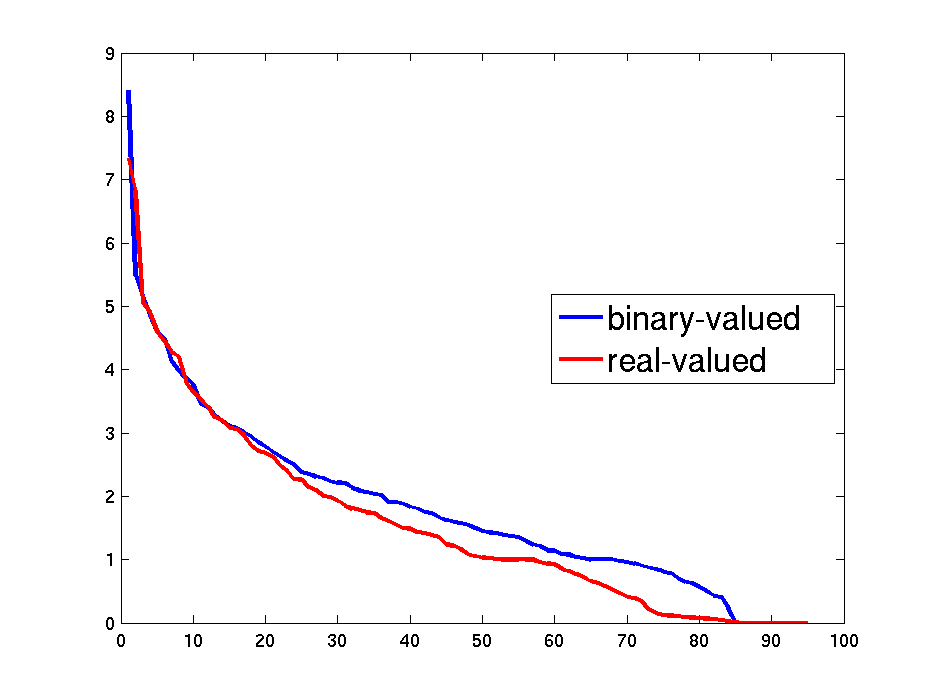
\includegraphics [scale=0.3] {sv-plot-creative.png}
	\label{fig:sv-creative}
	\end{subfigure}
	
\caption {Singular values of 4 products}
\label{fig:sv}
\end{figure}

\begin{figure}
\centering
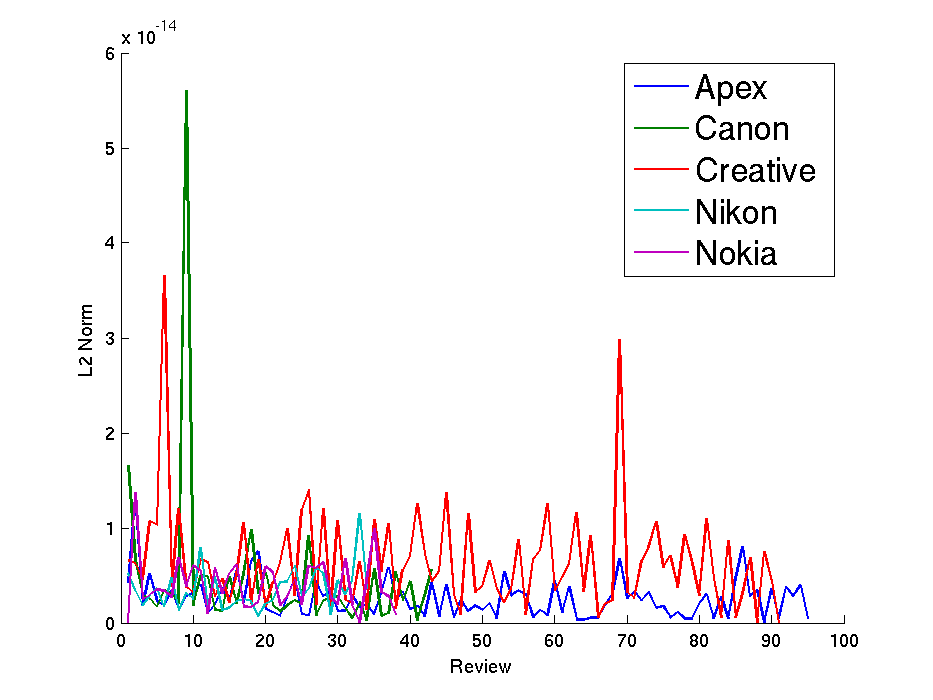
\includegraphics [width=\linewidth] {l2norm-plot-opinions.png}
\caption{L2 norms for product reviews}
\label{fig:l2norm-opinions}
\end{figure}

For example, review 8 for �Canon G3� has abnormally high opinion scores for the features mentioned in the review. Reviews 6 and 71 for �Creative� have high opinion scores and a large number of features, respectively.

In order to test the effectiveness of this method, I injected the Creative-Zen-Xtra review data (n=95) with data from different products to see if the method would detect the reviews of the different products. Since Creative is an MP3 player, I selected review data from a diaper product (�Diaper�), and review data from another mp3 player (�Micro�). The feature space of Diaper and the feature space of Creative are nearly disjoint, while the feature space of MicroMP3 would be nearly the same as Creative. Thus, the method should successfully detect the Diaper reviews but have difficulty detecting the MicroMP3 reviews. Figure \ref{fig:roc-creative-diaper-micro} shows the results of a threshold test (threshold varied from 9e-15 to 1e-16).

In each trial, the percentage of review data for each injected product so that 5-20\% of the reviews were for diapers and 95-80\% were for the Creative MP3 player. The method predicts the diaper reviews with reasonable success, with a 100\% TPR and 35\% FPR for a threshold of 3e-15 (reviews with a score less than 3e-15 were classified as the injected review) for the dataset with 10\% Diaper reviews. As expected, the method does not work well for the MicroMP3 product with a very similar feature space.

\begin{figure}
\centering
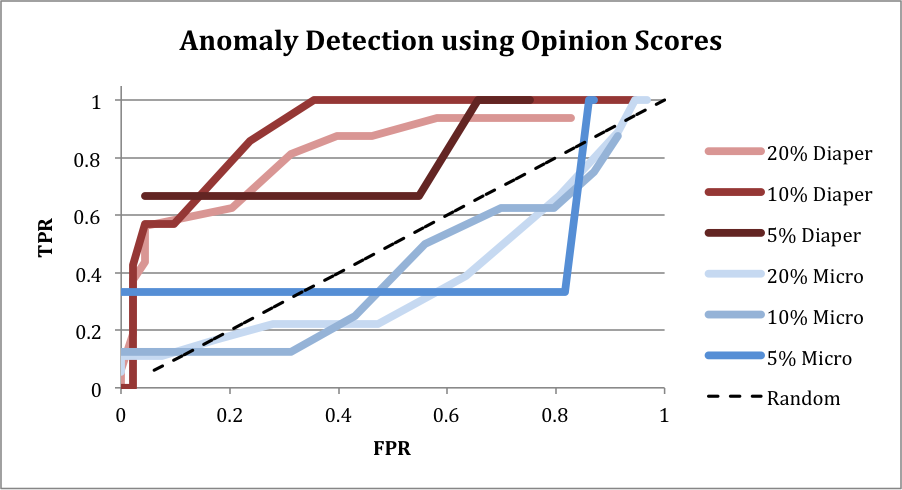
\includegraphics [width=\linewidth] {roc-plot-creative-diaper-micro.png}
\caption{Anomaly detection using opinion scores}
\label{fig:roc-creative-diaper-micro}
\end{figure}

The success of the method may be due to the fact that the L2 norm correlates with anomalous characteristics of the review. For instance, reviews with a large number of features or high average opinion score tend to have a high L2 norm. As Figure \ref{fig:correlation-l2norm-features-opinions} shows, the L2 norm has positive correlation with the number of features per review, and less pronounced but still positive correlation with the average opinion score per review (calculated using the dataset with 10\% diaper reviews).

\begin{figure}
\centering

	\begin{subfigure} {\linewidth}
	\centering
	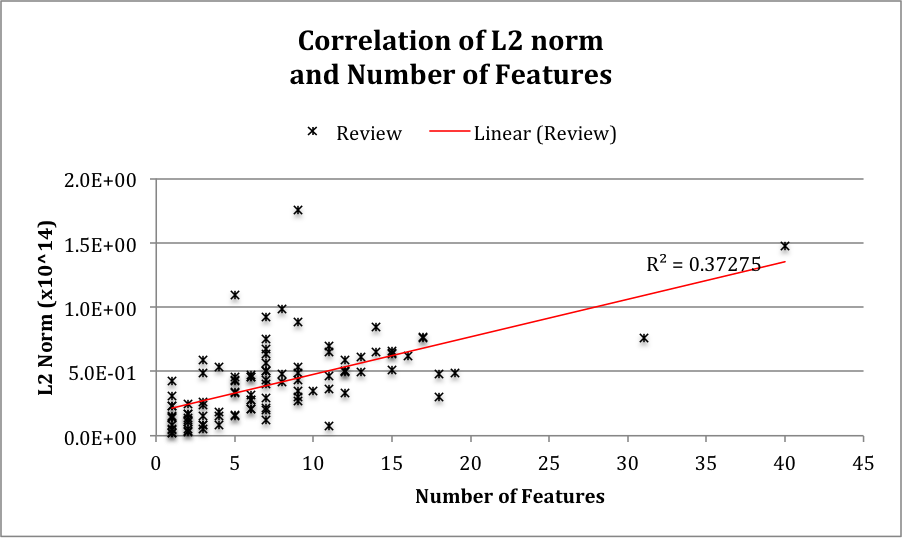
\includegraphics [width=\linewidth]{correlation-plot-l2norm-features-creative-diaper-10.png}
	\end{subfigure}
	
	\begin{subfigure} {\linewidth}
	\centering
	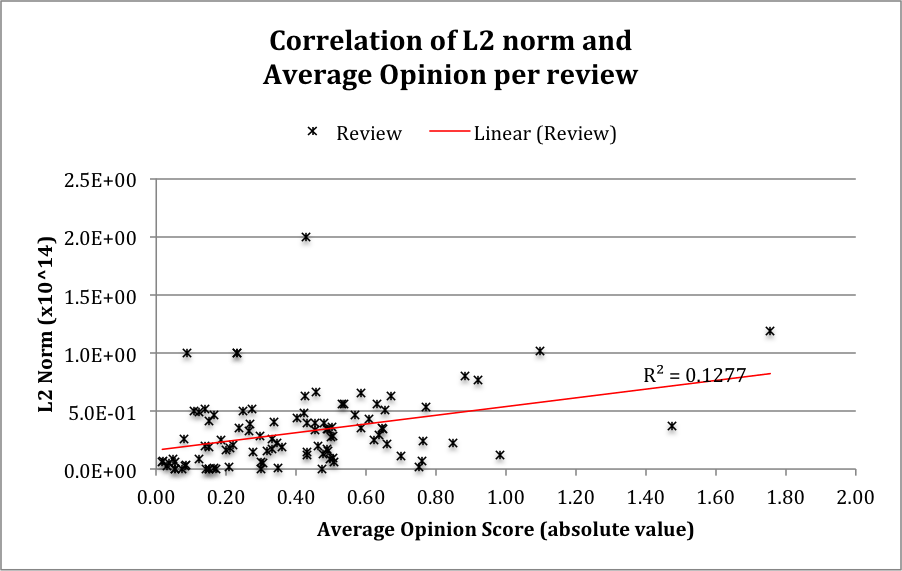
\includegraphics [width=\linewidth]{correlation-plot-l2norm-opinions-creative-diaper-10.png}
	\end{subfigure}
	
\caption{Correlation of L2 norm with \#features and average opinion score}
\label{fig:correlation-l2norm-features-opinions}
\end{figure}

Instead of using opinion scores, the method could also use TF-IDF scores, which reflects how important a particular word in a review. However, as I shall show, using opinion scores result in better performance.
The method for obtaining the TF-IDF data matrix is as follows: for each review, stem the text, remove stop words, and compute the TF-IDF of each unique word in the text. Finally, filter only the TF-IDF scores for the specified product attributes. Then each row of the data matrix is a review, and each column is a word in the review.

Figure \ref{fig:roc-tfidf-creative} shows a comparison of the L2 norm threshold test for the Creative MP3 reviews injected with Diaper reviews using opinion score features and using TF-IDF features. Here, the opinion score test performs much better than the TF-IDF test. Figure \ref{fig:roc-tfidf-creative} also shows the result of the TF-IDF test for the Creative MP3 reviews injected with MicroMP3 reviews. In this case, the TF-IDF test performs somewhat better than the opinion score test, but still close to random. This bad performance is expected because Micro MP3 and Creative MP3 are in the same product domain, so their feature spaces will be similar. 

\begin{figure}
\centering

	\begin{subfigure}{\linewidth}
	\centering
	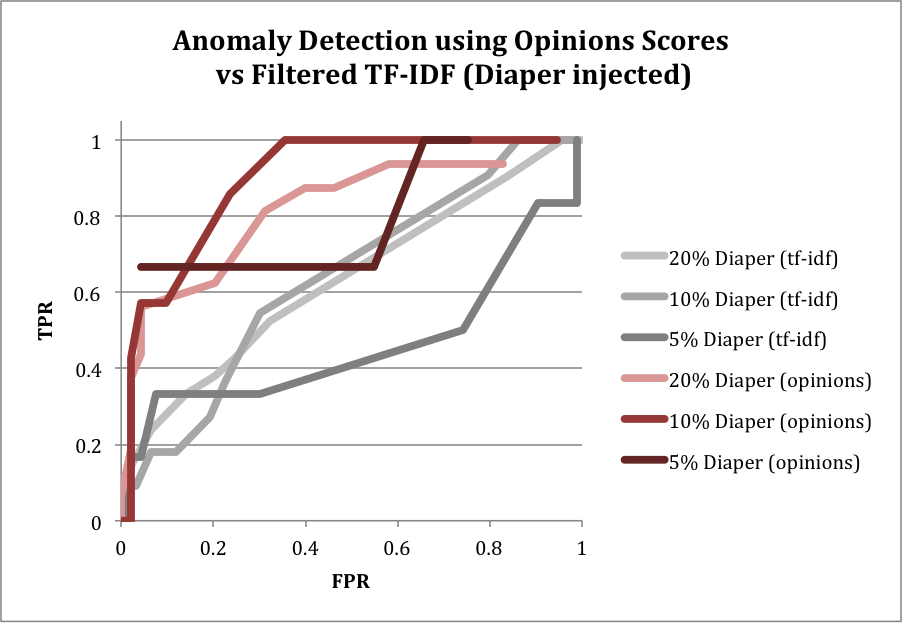
\includegraphics [width=\linewidth] {roc-plot-tfidf-creative-diaper.png}
	%\caption{Diaper injected}
	\label{fig:roc-tfidf-creative-diaper}
	\end{subfigure}

	\begin{subfigure}{\linewidth}
    	\centering
    	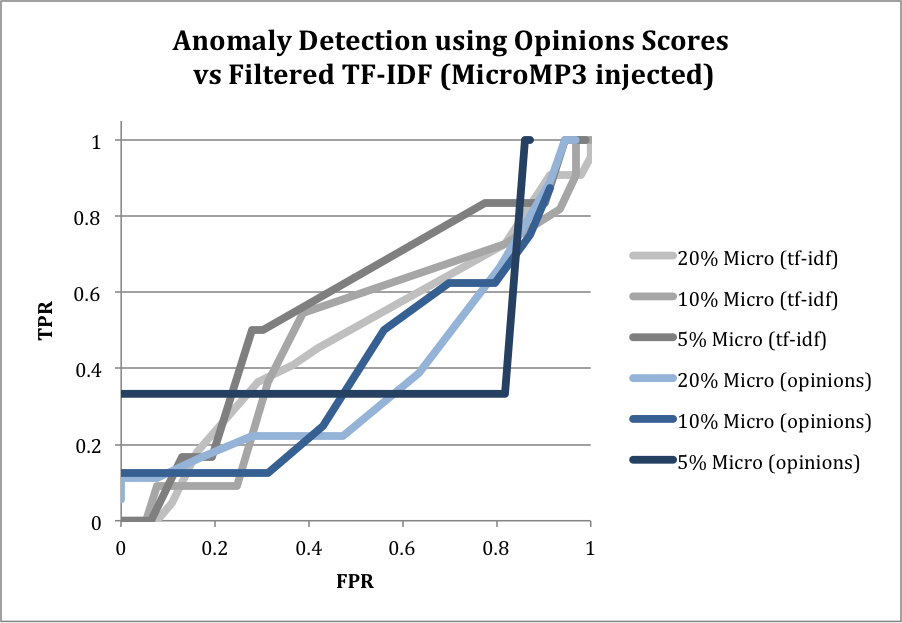
\includegraphics [width=\linewidth] {roc-plot-tfidf-creative-micro.png}
    	%\caption{MicroMP3 injected}
    	\label{fig:roc-tfidf-creative-micro}
   	\end{subfigure} 
	
\caption{Anomaly detection using opinion scores vs filtered TF-IDF}
\label{fig:roc-tfidf-creative}
\end{figure}

However, the TF-IDF measure actually does correlate with the L2 norm better than the opinion score measure correlates with the L2 norm. As Figure \ref{fig:correlation-l2norm-tfidf} shows, the L2 norm with the average TF-IDF score per review (using the dataset with 10\% diaper reviews) has a correlation coefficient of 0.30972 while the L2 norm with the average opinion score per review has a correlation coefficient of only 0.1277. The worse correlation of the number of features and opinion scores may indicate that these properties do not affect the anomaly detection as much as other properties in this dataset.

\begin{figure}
\centering
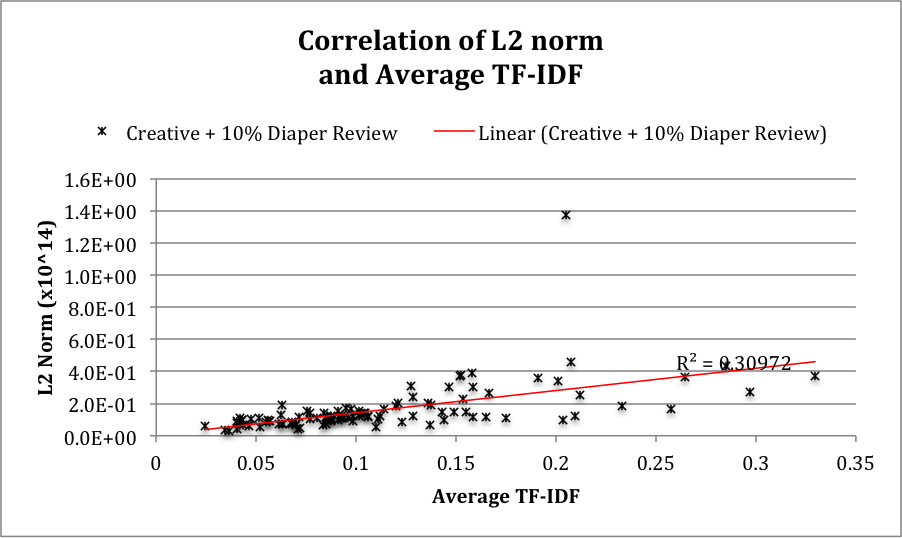
\includegraphics [width=\linewidth] {correlation-plot-l2norm-tfidf-creative-diaper-10.png}
\caption{Correlation of L2 norm with average TF-IDF}
\label{fig:correlation-l2norm-tfidf}
\end{figure}

In this paper, I have shown that an anomaly detection method using singular value decomposition and opinion scores of product attributes performs better than using TF-IDF values of product attributes.


\end{document}
